%-----------------------------------------------------------------------------
%
%               Template for sigplanconf LaTeX Class
%
% Name:         sigplanconf-template.tex
%
% Purpose:      A template for sigplanconf.cls, which is a LaTeX 2e class
%               file for SIGPLAN conference proceedings.
%
% Guide:        Refer to "Author's Guide to the ACM SIGPLAN Class,"
%               sigplanconf-guide.pdf
%
% Author:       Paul C. Anagnostopoulos
%               Windfall Software
%               978 371-2316
%               paul@windfall.com
%
% Created:      15 February 2005
%
%-----------------------------------------------------------------------------


\documentclass[nocopyrightspace, 10pt]{sigplanconf}

% The following \documentclass options may be useful:
%
% 10pt          To set in 10-point type instead of 9-point.
% 11pt          To set in 11-point type instead of 9-point.
% authoryear    To obtain author/year citation style instead of numeric.

\usepackage{natbib}
\usepackage{url}
\usepackage[squaren,thinqspace,binary]{SIunits}

\usepackage{hyperref}
\newcommand\fnurl[2]{%
  \href{#2}{#1}\footnote{\url{#2}}%
}

\let\fourth\relax               % Undefine a macro
\let\second\relax               % Undefine a macro
\let\degree\relax               % Undefine a macro
\let\cdot\relax                 % Undefine a macro
\usepackage{array}
\usepackage{amsmath}
\usepackage{amssymb}
%\usepackage{mathabx}
\usepackage{mathtools}
\usepackage{multirow}
\usepackage{bussproofs}
\usepackage{verbatim}
\usepackage{fancyvrb}

\usepackage{graphicx}
\usepackage{subcaption,placeins}
\usepackage{setspace}
%\usepackage[tight,footnotesize]{subfigure}
% \usepackage{subfigure}

\usepackage{listings}
\usepackage{xcolor}

% Display notes/comments with todonotes:
% \usepackage[disable]{todonotes} % notes/comments not showed
\usepackage[draft]{todonotes} % notes/comments showed

\newcommand{\fix}[1]{\texttt{\small #1}}
\lstset{
    inputencoding=utf8,
%    backgroundcolor=\color{white},
    tabsize=4,
    rulecolor=,
    upquote=true,
%    aboveskip={1.5\baselineskip},
    columns=fixed,
    showstringspaces=false,
    extendedchars=true,
    breaklines=true,
    prebreak = \raisebox{0ex}[0ex][0ex]{\ensuremath{\hookleftarrow}},
    frame=single,
    showtabs=false,
    showspaces=false,
    showstringspaces=false,
    basicstyle=\scriptsize\ttfamily,
    identifierstyle=\ttfamily,
    keywordstyle=\ttfamily\color[rgb]{0,0,1},
    commentstyle=\ttfamily\color[rgb]{0.133,0.545,0.133},
    stringstyle=\ttfamily\color[rgb]{0.627,0.126,0.941},
}



%\makeatletter
\lstdefinelanguage{llvm}{
  morecomment = [l]{;},
  morestring=[b]", 
  sensitive = true,
  classoffset=0,
  morekeywords={
    define, declare, global, constant,
    internal, external, private,
    linkonce, linkonce_odr, weak, weak_odr, appending,
    common, extern_weak,
    thread_local, dllimport, dllexport,
    hidden, protected, default,
    except, deplibs,
    volatile, fastcc, coldcc, cc, ccc,
    x86_stdcallcc, x86_fastcallcc,
    ptx_kernel, ptx_device,
    signext, zeroext, inreg, sret, nounwind, noreturn,
    nocapture, byval, nest, readnone, readonly, noalias, uwtable,
    inlinehint, noinline, alwaysinline, optsize, ssp, sspreq,
    noredzone, noimplicitfloat, naked, alignstack,
    module, asm, align, tail, to,
    addrspace, section, alias, sideeffect, c, gc,
    target, datalayout, triple,
    blockaddress, metadata
  },
  classoffset=1, keywordstyle=\color{purple},
  morekeywords={
    add, fadd, sub, fsub, mul, fmul,
    sdiv, udiv, fdiv, srem, urem, frem,
    and, or, xor,
    icmp, fcmp,
    eq, ne, ugt, uge, ult, ule, sgt, sge, slt, sle,
    oeq, ogt, oge, olt, ole, one, ord, ueq, ugt, uge,
    ult, ule, une, uno,
    nuw, nsw, exact, inbounds,
    phi, call, select, shl, lshr, ashr, va_arg,
    trunc, zext, sext,
    fptrunc, fpext, fptoui, fptosi, uitofp, sitofp,
    ptrtoint, inttoptr, bitcast,
    ret, br, indirectbr, switch, invoke, unwind, unreachable,
    malloc, alloca, free, load, store, getelementptr,
    extractelement, insertelement, shufflevector,
    extractvalue, insertvalue,
  },
  alsoletter=\%,
  keywordsprefix=\%,
}

%------------------------------------------------------------------------------
%\doublespacing
\begin{document}

%\titlebanner{banner above paper title}        % These are ignored unless
%\preprintfooter{preprint}   % 'preprint' option specified.

\title{Performance Analysis of Parallel Languages on Android}
%\subtitle{}

\authorinfo{Abdul Dakkak \and Cuong Manh Pham \and Prakalp Srivastava}
           {CS 598SVA - Heterogeneous Computing}
           % {University of Illinois at Urbana-Champaign}
           {\{dakkak, pham9, psrivas2\}@illinois.edu}

\conferenceinfo{CONF 'yy}{Month d--d, 20yy, City, ST, Country} 
\copyrightyear{20yy} 
\copyrightdata{978-1-nnnn-nnnn-n/yy/mm} 
\doi{nnnnnnn.nnnnnnn}

\maketitle
\todo[inline]{To do notes is enabled. Disable it to hide all notes}
%\category{CR-number}{subcategory}{third-level}

%\terms
%term1, term2

%\keywords
%keyword1, keyword2
\begin{abstract}
-- Abstract --

Our code is publicly available at \url{https://github.com/cmpham/RSBench}.

\end{abstract}

\section{Introduction}

Heterogeneous computing promises to address the rising power dissipation problem
of today's traditional homogeneous multi-core
systems. It provides the ability to integrate a variety of processing elements,
such as large and small general purpose cores, GPUs, DSPs, and custom or
semi-custom hardware into a single system. Applications that can efficiently use
the full range of available hardware reap significant energy
savings over conventional processors by executing portions of the code on the
device which optimized for it. This promise of performance along with power efficiency
has led mobile devices such as smartphones
and tablets, which deal with a variety of applications with limited battery
life, to move towards heterogeneous designs.

However, heterogeneity of hardware resources also has led to a diverse landscape
of different programming models, run-time systems, profiling and debugging tools
for application development. The differences are so deep that programmers are
often experts on only one class of device, e.g., an expert GPU programmer will
not have much DSP expertise and vice-versa. This is highly inefficient and
unproductive: we cannot expect applications to use a separate language for each
class of compute unit. If we want applications to use the full range of
available hardware to maximize performance or energy efficiency or both, the
programming environment has to provide common abstractions for available
hardware compute units.

The industry and the research community have been trying to solve this problem.
The recent development of RenderScript~\cite{wiki:RenderScript, RenderScript}
provides a framework for running computationally intensive tasks at a high
performance by using a specialized runtime for parallelizing work across all
processors available on the device, such as multi-core CPUs, GPUs, or DSPs.
RenderScript is therefore removing the burden of load balancing and memory
management from the programmer to the run-time, unlike other solutions such as
OpenCL, where the programmer has more control over the execution semantics of
the application ({\em the programmer decides which part of application would run
on which device and using which part of the memory heirarchy}).  In this fashion
RenderScript is making the computationally intensive part of the application,
that needs to be accelerated on specialized hardware, performance portable
across the various hardware compute units. Also, since the application is not
dependent on the existence and availability of a specific accelerator, the
application is portable across SoCs with varying combinations of compute units.

While such portability is a noble goal, RenderScript achieves it at the cost of
hiding hardware details from the programmer that are critical to good
performance on these accelerator. For example, in GPUs, the placement of data at
various levels of memory hierarchy is critical to good performance.  It is this
reason that most programming languages for GPUs, allow the programmer unlimited
control over memory management. RenderScript too can use GPUs for acceleration,
but completely hides the memory management from the programmer. In the
RenderScript model, application developers only define the part of the
application that needs to be accelerated, and the granularity at which data
needs to be partitioned, while the rest of the responsibilities of memory
management and work distribution among different compute units is handled by
RenderScript compiler and run-time.  This raises an important question of ``how
effective is the RenderScript compiler and run-time?'', which we plan to answer
by doing a comprehensive performance analysis of RenderScript.

Our code is publicly available at \url{https://github.com/cmpham/RSBench}.
Table~\ref{table:parboil} shows the porting status of each version of the
benchmarks in the Parboil Benchmark Suite.


\begin{table}[h]\small
\centering
\begin{tabu}{ | l |[1.5pt] c | c | c | c | c | c |}
    \hline 
    Benchmark & \multicolumn{6}{c|}{Implementations} \\ \cline{2-7}
                      & NC & OMP & J & JT & OCL & RS \\ \tabucline[1.5pt]{-}
    VectorAdd         & C & C   & C    & C      & C      & C \\ \hline
    SGEMM             & C & C   & C    & C      & C      & C \\ \hline
    Stencil           & C & C   & C    & C      & C      & C \\ \hline
    CUTCP             & N & N   & C    & C      & C      & C \\ \hline
    MRI-Q             & N & N   & C    & C      & C      & C \\ \hline
    TPACF             & B & B   & C    & C      & C      & C \\ \hline
    Histogram         & C & B   & C    & C      & C      & C \\ \hline
    BFS               & \multicolumn{6}{c|}{N} \\ \hline
    MRI-G             & \multicolumn{6}{c|}{N} \\ \hline
    SAM               & \multicolumn{6}{c|}{N} \\ \hline
    SPMV              & \multicolumn{6}{c|}{N} \\ \hline
    LBM               & \multicolumn{6}{c|}{N} \\ \hline
    \hline
\end{tabu}
\caption{Parboil Benchmark Porting Status. \textbf{NC} : Native C; \textbf{OMP}
: Native C with OpenMP; \textbf{JT}: Threaded Java; \textbf{OCL} : OpenCL;
\textbf{RS}: RenderScript; \textbf{C}: Completed; \textbf{N} : No
Implementation; \textbf{B} : a bug causes the benchmark to crash.}
\label{table:parboil}
\end{table}


\section{Motivation and Background}
\todo[inline]{Assuming Introduction has a sentence or two about the
programmability problem.}


Heterogeneity of hardware resources has led to a diverse landscape
of different programming models, run-time systems, profiling and debugging tools
for application development. The differences are so deep that programmers are
often experts on only one class of device, e.g., an expert GPU programmer will
not have much DSP expertise and vice-versa. This is highly inefficient and
unproductive: we cannot expect applications to use a separate language for each
class of compute unit. If we want applications to use the full range of
available hardware to maximize performance or energy efficiency or both, the
programming environment has to provide common abstractions for available
hardware compute units.

OpenCL and RenderScript have been proposed to solve this problem. They are
designed to accelerate data parallel computation intensive part of application
code by allowing workload to be executed on multiple processing cores, GPUs,
DSPs or a combination of these. Here we give a brief overview of OpenCL and
RenderScript.

\subsection{OpenCL}
OpenCL was initiated by Apple Inc. and is managed by the Khronos
Group~\cite{Khronos:url}. It allows the application developers to write
data parallel computation intensive parts of their application for an abstract
hardware model, without using low level hardware specific function calls.

An OpenCL application is composed of two parts: an OpenCL host program and a
set of one or more kernels. The kernels, written in restricted C99 syntax,
specify functions that are to be executed in data parallel fashion. The OpenCL
host program identifies the device on which the OpenCL kernel would be
executed, sets up the environment, allocate memory on the device, copy data
into the device memory and enqueue the kernel execution on the device.

In the Android world, where all application execute on Dalvik virtual machine,
an application using OpenCL has a third component as well. This is the Java
host code which would initialize the application, read in the inputs and use
JNI calls to invoke OpenCL host code.

OpenCL is designed to be portable across a wide range of devices. However,
developers often use hardware specific parameters such as the size of OpenCL
work-group, shared memory size to obtain better performance on specific
hardware. This harms the portability of OpenCL application kernel code.

\subsection{RenderScript}
RenderScript was released by Google as an official computing framework in
2011~\cite{RederScript:url}. The motivation behind RenderScript is to provide
performance and portability across SoC architectures to RenderScript
applications.

A RenderScript application consists of three parts: (1) Java application host
code written by the developer that runs on Dalvik VM, (2) RenderScript code
written in restricted C99 syntax containing one or more kernels, and (3)
auto-generated Java code that helps application host code to communicate with
RenderScript kernel code, allowing functions such as memory binding between the
host program and the kernels.

RenderScript compilation flow is shown in Figure~\ref{fig:RSCompilation}.
First, \fix{llvm-rs-cc} utility is used to compile RenderScript kernels to
LLVM~\ref{LLVM:url} bitcode (\fix{*.bc extension}) files. LLVM bitcode is LLVM
intermediate representation having backend support for a wide range of hardware
devices including general purpose processors, GPUs and DSPs. All OpenCL
compilers too use a subset of LLVM IR as intermediate representation, thus
making it a natural choice for RenderScript IR which has portability as one of
its primary goal. During compilation of RenderScript kernels, \fix{llvm-rs-cc}
also generates the corresponding reflected Java classes of the kernels.
Thereafter, the application host code, the reflected Java classes and bitcode
are bundled together into the Android application package (\fix{*.apk} file),
which is installed on the Android device. During execution, the RenderScript
runtime invokes \fix{libbcc}, RenderScript back-end compiler to translate
bitcode into appropriate machine code.


\todo[inline]{Programmability Challenge: Elaborate on that}
\todo[inline]{LLVM IR code snippet}
\lstinputlisting[language=llvm, caption=Bitcode representation of RenderScript kernel]{code/average.ll}
\lstinputlisting[language=llvm, caption=NVVM representation of CUDA kernel]{code/simple-gpu.ll}
\lstinputlisting[language=llvm, caption=SPIR representation of OpenCL kernel]{code/average-opencl.ll}

The industry and the research community have been trying to solve this problem.
The recent development of RenderScript~\cite{wiki:RenderScript, RenderScript}
provides a framework
for running computationally intensive tasks at a high performance by using a
specialized runtime for 
parallelizing work across all processors available on the device, such as
multi-core CPUs, GPUs, or DSPs. RenderScript is therefore removing the
burden of load balancing and memory management from the programmer to the run-time, unlike other
solutions such as OpenCL, where the programmer has more control over the
execution semantics of the application ({\em the programmer decides which part
of application would run on which device and using which part of the memory heirarchy}).
In this fashion RenderScript is
making the computationally intensive part of the application, that needs to be
accelerated on specialized hardware, performance portable across the various hardware compute
units. Also, since the application is not dependent on the existence and
availability of a specific accelerator, the application is portable across SoCs
with varying combinations of compute units.

While such portability is a noble goal, RenderScript achieves it at the cost of
hiding hardware details from the programmer that are critical to good
performance on these accelerator. For example, in GPUs, the placement of data at
various levels of memory hierarchy is critical to good performance.
It is this reason that most programming languages for GPUs, allow the programmer
unlimited control over memory management. RenderScript too can use GPUs for acceleration, but
completely hides the memory management from the programmer. In the RenderScript
model, application developers only define the part of the application that needs
to be accelerated, and the granularity at which data needs to be partitioned,
while the rest of the responsibilities of memory management and work distribution
among different compute units is handled by RenderScript compiler and run-time.
This raises an important
question of ``how effective is the RenderScript compiler and run-time?'', which
we plan to answer by doing a comprehensive performance analysis of RenderScript.



\section{Methodology}


\subsection{Performance Analysis}


\subsection{Power Analysis}


Since Android does not offer a way to capture processor usage information
  programatically, we use the Trepn tool by Qualqomm to capture the
  data for us and save it into a {\tt csv} file.   
Trepn, which is limited to Qualcomm based chipsets, reads internal processor
  counters as well as power rail information, both of which are not otherwise
  available programatically.
We set Trepn to read the counters every $100ms$ and measure the load and power
  usage seperatly to decrease the overhead of the profiler.
To reduce overhead, Trepn measure the processor usage information every $100ms$, both
  the frequency and the load are measured sequentially, we therefore need to 
  correct that when parsing the {\tt csv} file.

  
First, we parse each processor reading along with the time stamp for reading
  the file.
Next, we interpolate the measured data (we use linear interpolant) and
  evaluate the interpolant at the application state times (these are the
  times Trepn recieved a signal from our application and correspond to
  timed blocks of code).
We then multiply the load by the frequency, and rescale all the CPU and GPU data (we perform the rescaling on the CPU and GPU seperatly).
Trepn can have measurment errors, resulting in infinite numbers.
To make sure that these do not skew the plots, we clip the range of possible processor reading to be between 1 and the the $0.99$th quantile of the data.
While efforts have been taken to reduce the profiler's overhead, it still 
  ocupies around a $10\%$ overhead.


\section{Implementation}

\subsection{The RSBench Framework Structure}

\begin{figure}[t!]
\centering
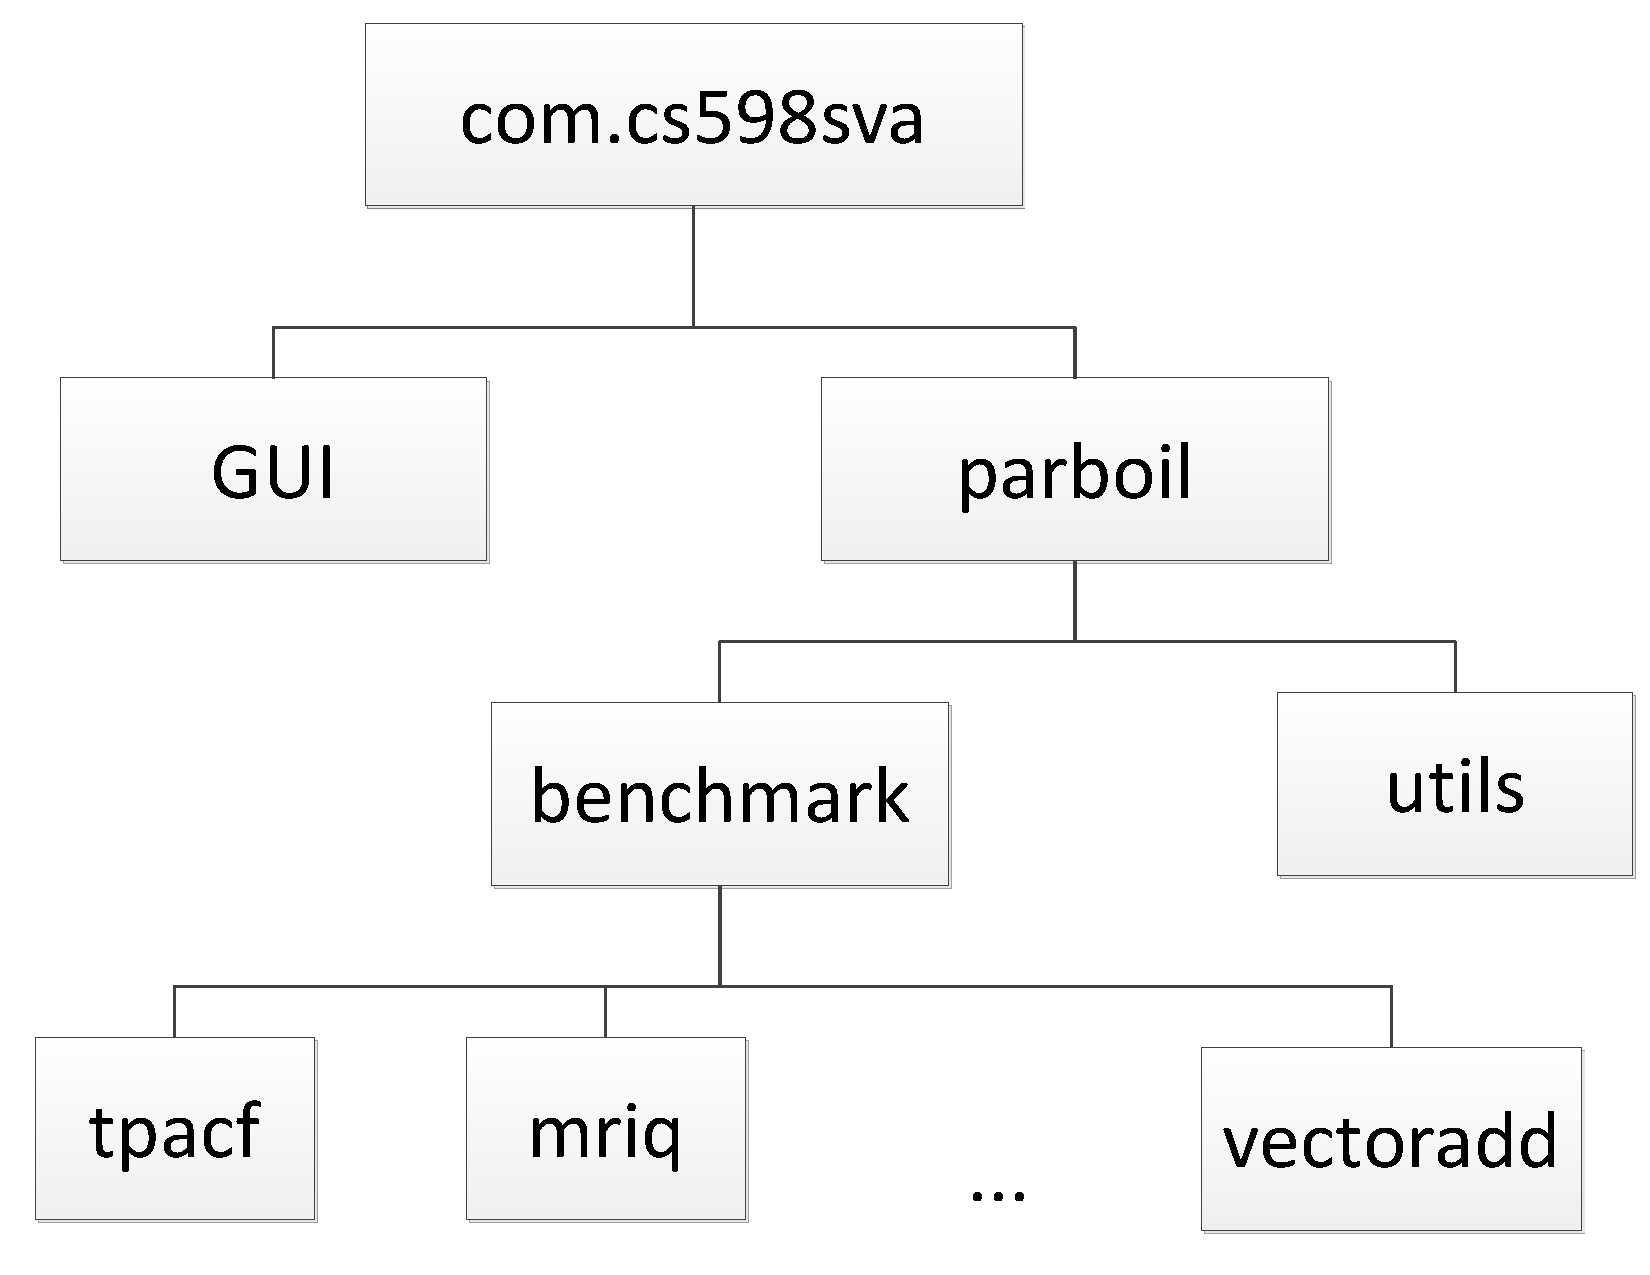
\includegraphics[scale=0.65]{figs/package_diagram.pdf}
\caption{RSBench Java package structure.}
\label{fig:package_structure}
\centering
\end{figure}


\begin{figure}[t!]
\centering
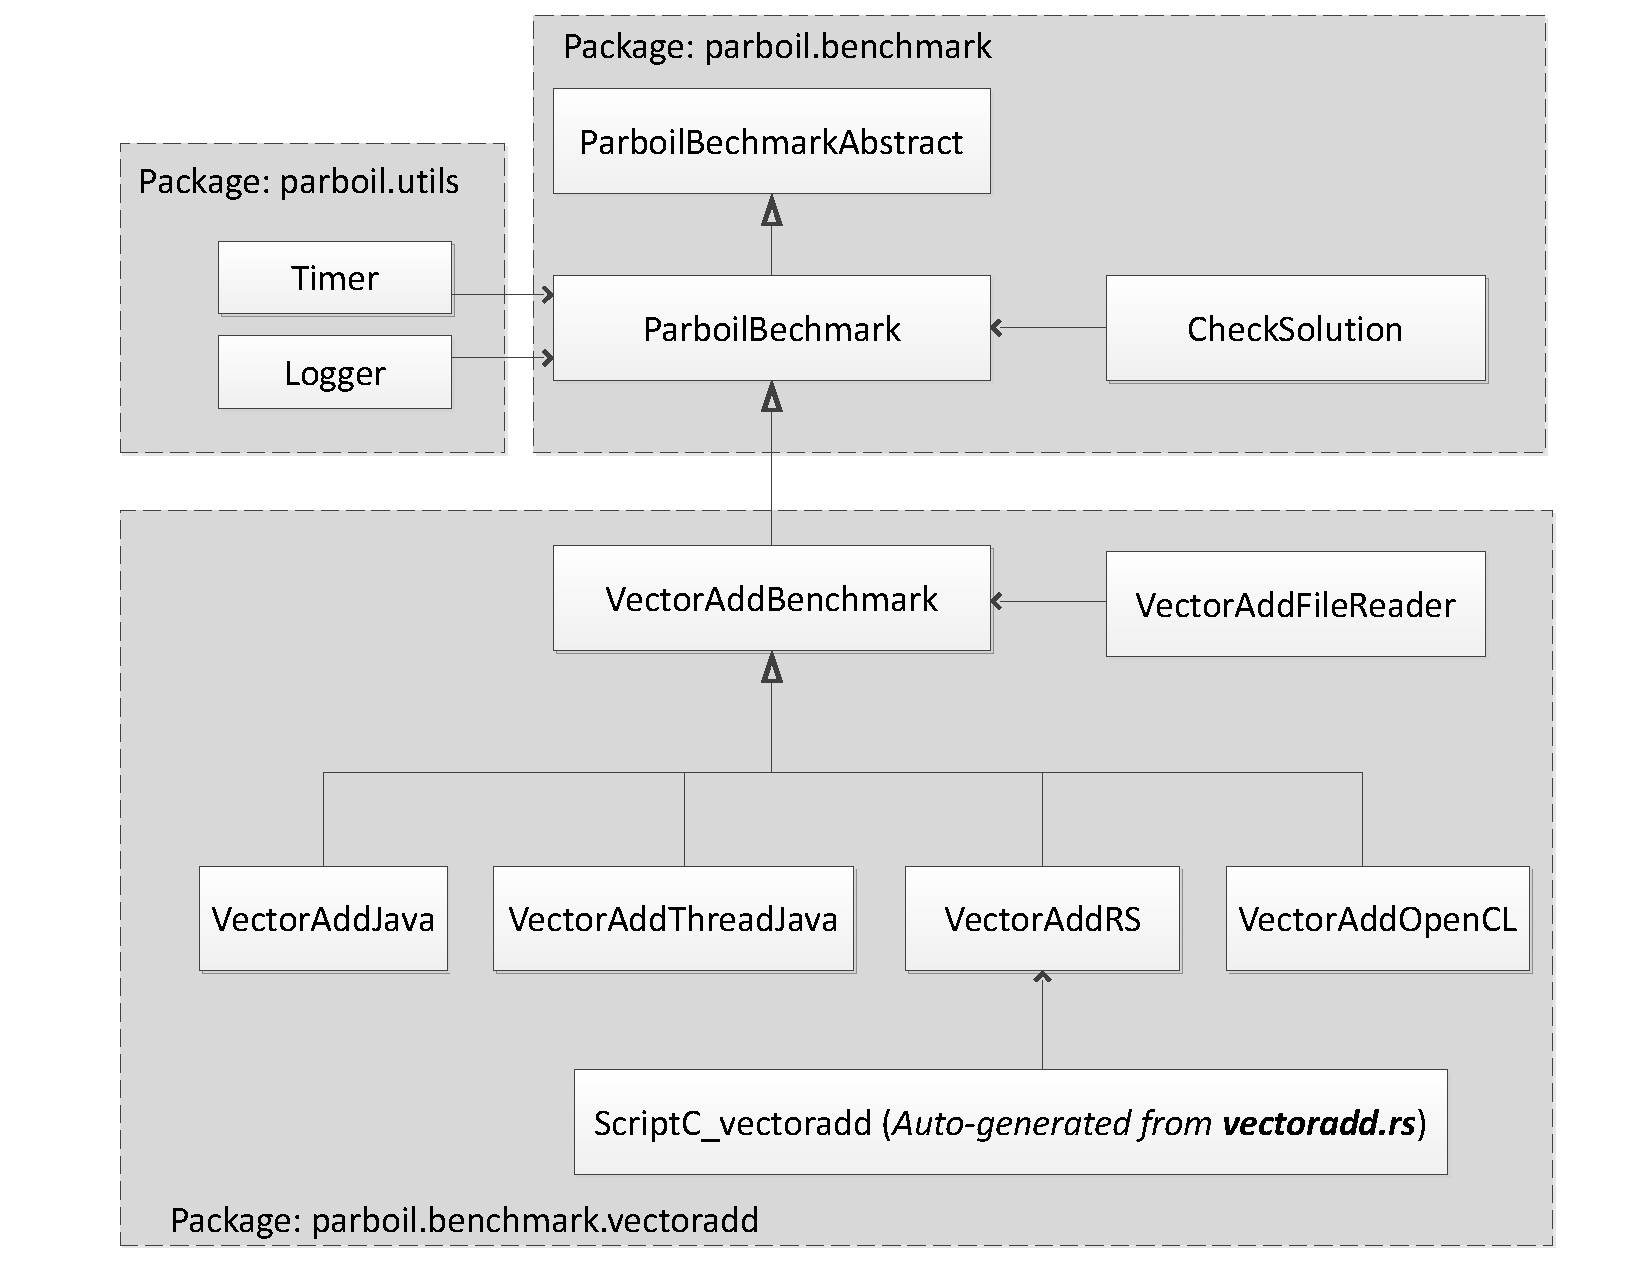
\includegraphics[scale=0.5]{figs/vectoradd_class_diagram.pdf}
\caption{Class diagram of the VectorAdd benchmark.}
\label{fig:class_diagram}
\centering
\end{figure}

In order to facilitate the development of the benchmarks, we designed a
framework, called RSBench, which contains (i) a hierarchy of the benchmarks, e.g.,
all different implementations of the same benchmark are group together, and
(ii) utilities functions that support measuring and recording the results.
Figure \ref{fig:package_structure} depicts the overview of the framework by mean
of the Java package structure. Figure \ref{fig:class_diagram} provides a closer
view at the organization of the classes related to the VectorAdd benchmark.

At a high level, we split the development of the graphical user interface (GUI),
from the development of each of the benchmarks, under the \fix{GUI} package and
the \fix{parboil} package in Figure \ref{fig:package_structure}, respectively.
At this stage, the GUI is simply to allow users to start running the benchmarks,
and to display the status of the benchmark execution, e.g., in which stage a
benchmark is running, and whether a benchmark has executed successfully or
failed at the end. In the future, more features will be added, such as
displaying the final scores of the device.

The \fix{parboil} Java package is the core of the project. In this package, we
identified the common utility functions, such as timing- and logging-related
functions, that are used across all the benchmarks. Those functions are grouped
in classes, e.g., \fix{Timer} and \fix{Logger}, and implemented in the
\fix{utils} package. Each benchmark, e,g., \fix{bfs} or \fix{cutcp}, is
implemented in a separate package under the \fix{benchmark} package.  Figure
\ref{fig:class_diagram} depicts the class diagram of the VectorAdd benchmark.
Other benchmarks have the same class structure. In order to implement a
benchmark, we just need to inherit for the \fix{ParboiBenchmark} class, which
layouts a common skeleton. For each benchmark, we have to implement a class to
read the input, for example \fix{VectorAddFileReader} class in this case. Each
computational kernel, e.g., for Java, threaded Java, RenderScript, or OpenCL, is
implemented in a separate class, e.g., \fix{VectorAddJava},
\fix{VectorAddThreadedJava}, \fix{VectorAddRS}, or \fix{VectorAddOpenCL},
respectively. These classes inherit from the parent class of the benchmark,
which is the \fix{VectorAddBenchmark} in this case. This hierarchical design
maximize the code reuse between benchmarks, and between computation kernel.  It
also allows for a consistent interface to run the benchmarks.


\subsection{Utility Functions}
\subsubsection{Timer}
The \fix{Timer} class is an important utility in our benchmark. It
determines the accuracy and flexibility of our measurement. The \fix{Timer}
class utilizes Android's \fix{SystemClock}, which provides real-time clock at
nanosecond resolution. Each \fix{Timer} object consists of a dynamic list of
\fix{TimerElement} objects. Each \fix{TimerElement} object is a measure of a
particular execution segment, e.g., allocation time, setup time, and compute
time. In order to create a new \fix{TimerElement}, we just need to invoke the
\fix{Timer.start(category, message)} method at the beginning of the execution
segment we wish to measure (here category is a user defined category such as
``Compute'' or ``Setup'', while message is a message that further refines the
category such as ``Allocating temporary data structures''). At the end of the
execution segment, we need to invoke the \fix{Time.stop()} method. The
time-stamp and elapsed time will be automatically computed and recorded.
The \fix{Timer} class also can dump all the recorded \fix{TimerElement} to a
SQLite database or serialize it to the JSON format for conveniently storing and
parsing the results.

If a benchmark is run multiple times, for example, we run the compute part 100
times for each small benchmark, and five times for each big benchmark in our
currently analysis, then the \fix{Timer} has a function to aggregate the results
to output the average time across runs.  Currently, we do not exercise that code
and we leave the statistical analysis to the parser and visualizer.

\subsubsection{Output to Database}

Unlike Parboil, which outputs the times to {\tt stdout}, we output our data into
a SQLite database.  This affords us a few things.  First, since data is
outputted in the specified columns, we do not have to re-parse the output data.
Second, timing information can be shared easily by copying the database.
Finally, we can store more than just timing information -- for example we also
store which machine the time has been taken on as well as which runtime is being
used.  Since writing to flash is extensive, all timing data is stored in memory
and after the benchmark has run it is inserted into the database. 

\subsubsection{Load/Power Profiler}

Since Android does not offer a way to capture processor usage information
programatically, we use the Trepn tool by Qualqomm to capture the data for us
and save it into a {\tt csv} file.   Trepn, which is limited to Qualcomm based
chipsets, reads internal processor counters as well as power rail information,
both of which are not otherwise available programatically.  We set Trepn to read
the counters every $100ms$ and measure the load and power usage seperatly to
decrease the overhead of the profiler.  To reduce overhead, Trepn measure the
processor usage information every $100ms$, both the frequency and the load are
measured sequentially, we therefore need to correct that when parsing the {\tt
csv} file.

First, we parse each processor reading along with the time stamp for reading the
file.  Next, we interpolate the measured data (we use linear interpolant) and
evaluate the interpolant at the application state times (these are the times
Trepn recieved a signal from our application and correspond to timed blocks of
code).  We then multiply the load by the frequency, and rescale all the CPU and
GPU data (we perform the rescaling on the CPU and GPU seperatly).  Trepn can
have measurment errors, resulting in infinite numbers.  To make sure that these
do not skew the plots, we clip the range of possible processor reading to be
between 1 and the the $0.99$th quantile of the data.  While efforts have
been taken to reduce the profiler's overhead, it still ocupies around a
$10\%$ overhead.


\subsection{Implementing Computational Kernels}
\label{sec:imple_RS}

\begin{table}[tp]\small
\centering
\begin{tabular}{ | l | c |}
    \hline 
    Language      & Line Count \\ \hline
    Java          & 7549       \\ \hline
    RenderScript  & 1000       \\ \hline
    JNI/C++       & 2048       \\ \hline
    OpenCL        & 480        \\ \hline
\end{tabular}
\caption{RSBench project line count breakdown.}
\label{table:breakdown}
\end{table}

Table~\ref{table:breakdown} shows the numbers of line-of-code (LOC) broken down
into different types of programming languages in the RSBench project. The next
sub-sections describe the process of implementing different types of computational
kernels for each benchmark.

\subsubsection{RenderScript Kernels}
%This section describes the general steps to write a computation kernel in
%RenderScript for our benchmark.

By design, each RenderScript kernel produces an \textit{element} of the output.
It is up to developers to define the granularity of an element. For example, in
the VectorAdd benchmark, an output element can be one, or two, or three array
elements of the output vector. This granularity essentially determines the
parallelism of the written RenderScript code. In our benchmarks, we select the
finest granularity of the output element, e.g., one array element in this case,
to implement our RenderScript kernel.

In order to support this model, the RenderScript framework provides APIs to (i)
define the type of \fix{Element} for both input and output of RenderScript
kernels, and (ii) pack \fix{Element}s into \fix{Allocation}, which is the data
structure that is used to pass data back and forth between regular Java code and
RenderScript code.

A significant effort of our work is to determine efficient ways to convert input
data from original structure to the \fix{Allocation} structure with appropriate
\fix{Element} type. This conversion is also reflected at runtime through the
\textit{setup} time category of RenderScript execution.

After data has been packed into \fix{Allocation} objects, we move to write
RenderScript code in C99 format. The code needs to be placed in a specific file
with the $.rs$ extension and a proper header, so that the Android Development
Tools (ADT) can automatically generate a wrapper Java class for it. The
auto-generated Java class provides interfaces to invoke the RenderScript code
from Java code.

\subsubsection{Native Kernels}

The Android operating system requires that C, OpenMP, and OpenCL kernels have to
be invoked through Java Native Interface (JNI).  The C and OpenMP versions of
the code have been taken from Parboil with minimal modifications.  Aside from
wrapping the code via JNI so it is callable from within Java, little
modification was done to the C and OpenMP code.

The OpenCL kernels are lifted from the parboil benchmark suite with no
modifications.  We use the \fix{base} implementation of OpenCL --- this a
platform agnostic unoptimized implementation.  Unlike the Parboil benchmark
suite, we write the OpenCL host code using the C++ OpenCL API, this simplifies
some of the code and affords us more code reuse oportunities.

To allow devices with no OpenCL support to make use of the C and OpenMP
implementations, we generate 3 libraries (one for C, OpenMP, and OpenCL).  Each
library is then loaded and called from with its class implementation.


\section{Benchmarks}
\label{sec:benchmarks}

We extend the Parboil benchmark suite to run on Android devices.
Table~\ref{table:parboil} shows the porting status of each version of the
benchmarks in the Parboil Benchmark Suite.


\begin{table}
\centering
\begin{tabu}{ | l | c | c | c | c | c | c |}
    \hline 
    Benchmark & \multicolumn{6}{c|}{Implementations} \\ \cline{2-7}
                      		   & NC & OMP & J    & JT     & OCL    & RS\\ \hline
    \textbf{VectorAdd}         & C  & C   & C    & C      & C      & C \\ \hline
    \textbf{SGEMM}             & C  & C   & C    & C      & C      & C \\ \hline
    \textbf{Stencil}           & C  & C   & C    & C      & C      & C \\ \hline
    \textbf{CUTCP}             & N  & N   & C    & C      & C      & C \\ \hline
    \textbf{MRIQ}             & N  & N   & C    & C      & C      & C \\ \hline
    \textbf{TPACF}             & B  & B   & C    & C      & C      & C \\ \hline
    \textbf{Histogram}         & C  & B   & C    & C      & C      & C \\ \hline
    \textbf{BFS}               & \multicolumn{6}{c|}{N} \\ \hline
    \textbf{MRIG}             & \multicolumn{6}{c|}{N} \\ \hline
    \textbf{SAM}               & \multicolumn{6}{c|}{N} \\ \hline
    \textbf{SPMV}              & \multicolumn{6}{c|}{N} \\ \hline
    \textbf{LBM}               & \multicolumn{6}{c|}{N} \\ \hline
    \hline
\end{tabu}
\caption{Parboil Benchmark Porting Status. \textbf{NC}: Native C; \textbf{OMP}:
Native C with OpenMP; \textbf{JT}: Threaded Java; \textbf{OCL}: OpenCL;
\textbf{RS}: RenderScript; \textbf{C}: Completed; \textbf{N}: No Implementation;
\textbf{B}: a bug causes the benchmark to crash.}
\label{table:parboil}
\end{table}

In this section, we give an overview of the benchmarks implemented along with 
	the dataset sizes we used when profiling the results.
While the Parboil benchmark suite represents scientific workloads, we expect them to be 
	representative of future Android applications --- given that we already 
	see laptops using Android as their OS.

\subsection{VectorAdd}

The VectorAdd benchmark adds two floating point vectors with $8K$ elements.
Compared to other benchmarks, VectorAdd has a very high memory to compute ratio.
The benchmark is therefore not a fit for parallelization, but we use it to examine
  the overhead behavior.

\subsection{SGEMM}

The SGEMM benchmark multiplies two matrices $A$ and $B$ produces an output $C$.
Matrix $A$ is of dimension $128 \times 96$ and $B$ is of dimension $96 \times 160$.
Matrix $A$ is stored in the row major format, while $B$ is stored in the column major format ---
	we therefore do not need to transpose $B$ to make effective use of the cache.

The OpenMP code uses the \fix{\#pragma omp parallel for shared(A, B, C) collapse(2)}
	pragma, in which, based on the processor utilization,
	the Android compiler was not able to parse as valid OpenMP code.
Therefore, the OpenMP code for SGEMM is equivalent to the serial C code.

\subsection{TPACF}

The TPACF benchmark analyzes the angular distribution of astronomical objects.
The algorithm computes the distances between all pairs of coordinates in a dataset
	and then performs histogramming.
The results are collected in three histograms which are then cross-correlated to find
	the statistical spatial distribution of the astronomical bodies.
For our analysis, we use $100$ datasets, each containing $487$ coordinates.

\subsection{MRIQ}

The MRIQ benchmark computes a non-uniform 3D inverse-Fourier-transform, representing a calibration matrix.
The calibration matrix is used to perform 3D image reconstruction from MRI data which is 
	presented in a non-Cartesian space.
The input dataset is of size $32 \times 32 \times 32$ containing trajectory information in $3$D
	as direction parameter in $2$D.

\subsection{Stencil}

The Stencil benchmark computes a 7 point stencil of an input volume. 
The input volume has dimension $128 \times 128 \times 32$.
Each kernel performs a standard 7 point stencil: accessing the $6$ adjacent voxels,
	scaling and then adding them to the current voxel.
The result is then placed in the output buffer.

\subsection{Histogram}

The Histogram benchmark computes the histogram of an input image.
The input image is of size $996 \times 1040$ and compute a 
	histogram of size $256$.
Each bin in the histogram saturates at the value $255$.

Unlike the other parallel implementations, which use atomics, both the
	threaded Java and OpenMP implementations use privatizations.
Private histogram copies are allocated, each thread 
	operates on its own private copy, and once the threads finish, the
	master thread aggregates the results.


\section*{Analysis}
\label{sec:analysis}

The emulator is used to perform the debugging (although it does not seem to be able to run RenderScript code).
To run the code, we are using two devices for the analysis.
The first is a Nexus 7 with the following specs:

\begin{verbatim}
    CPU: Qualcomm Snapdragon S4 Pro, 1.5GHz
    GPU: Adreno 320, 400MHz
    Memory - 2 GB
    Storage 32 GB
\end{verbatim}

The second is a Samsung Galaxy Nexus with the following specs:

\begin{verbatim}
    CPU: ARMv7, 2 cores, 1200 Mhz, SIMD NEON
    Memory: 694, JVM max: 96 MB
    GPU: PowerVR SGX 540.
\end{verbatim}


\subsection*{Perliminary Results}

While we do have implementations for 3 out of the 4 benchmarks we promised in the proposal schedule,
  our results only show part of those.
The data has not been fully analyzed, but we can give some perliminary insights into the expected
  results.


\begin{figure}[t!]
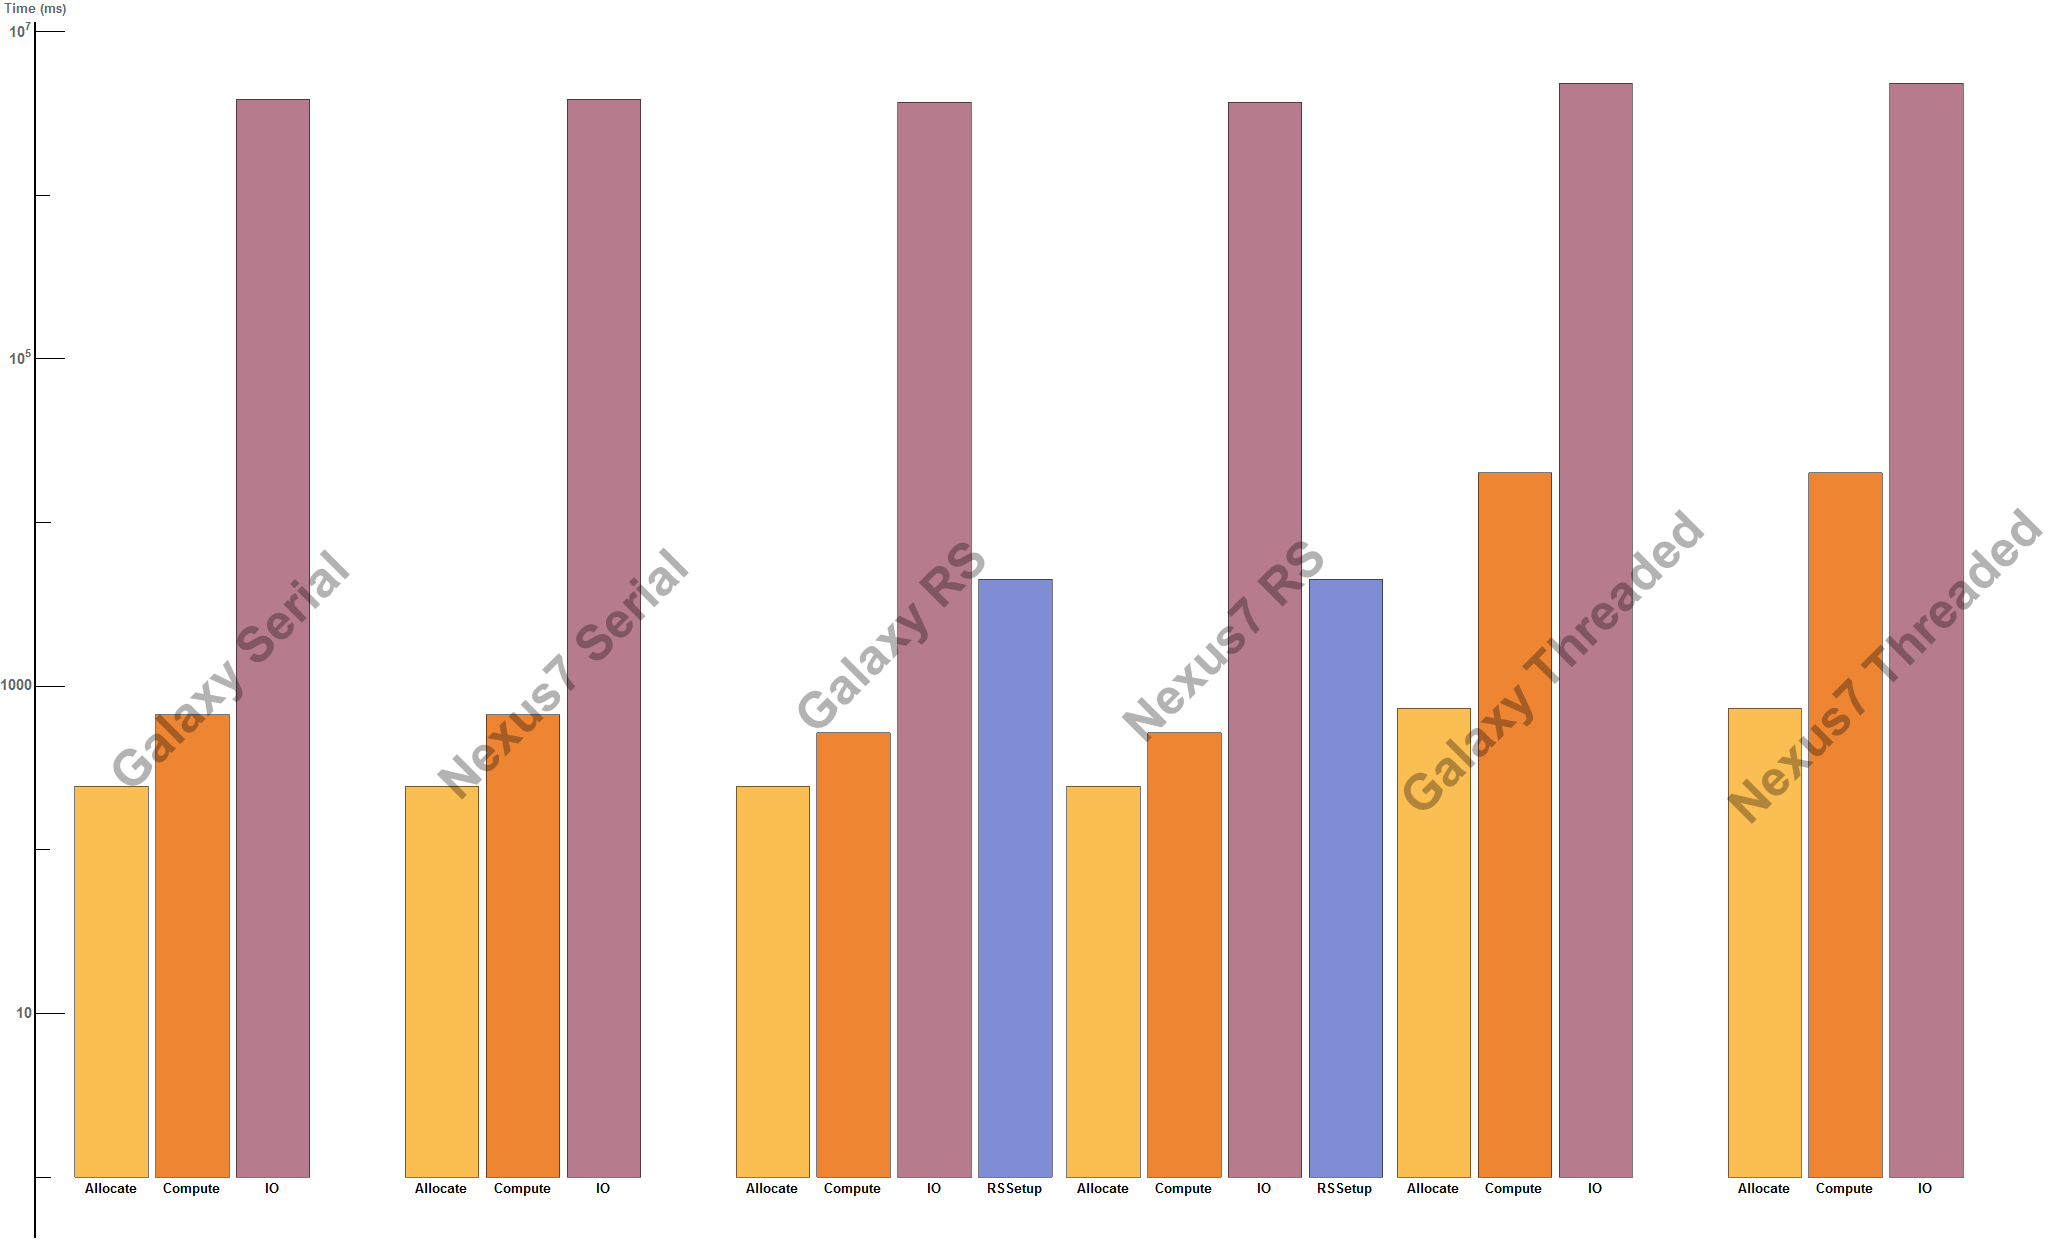
\includegraphics[scale=0.125]{VectorAdd.png}
\caption{VectorAdd Benchmark.}
\label{fig:vecadd}
\centering
\end{figure}



\begin{figure}[t!]
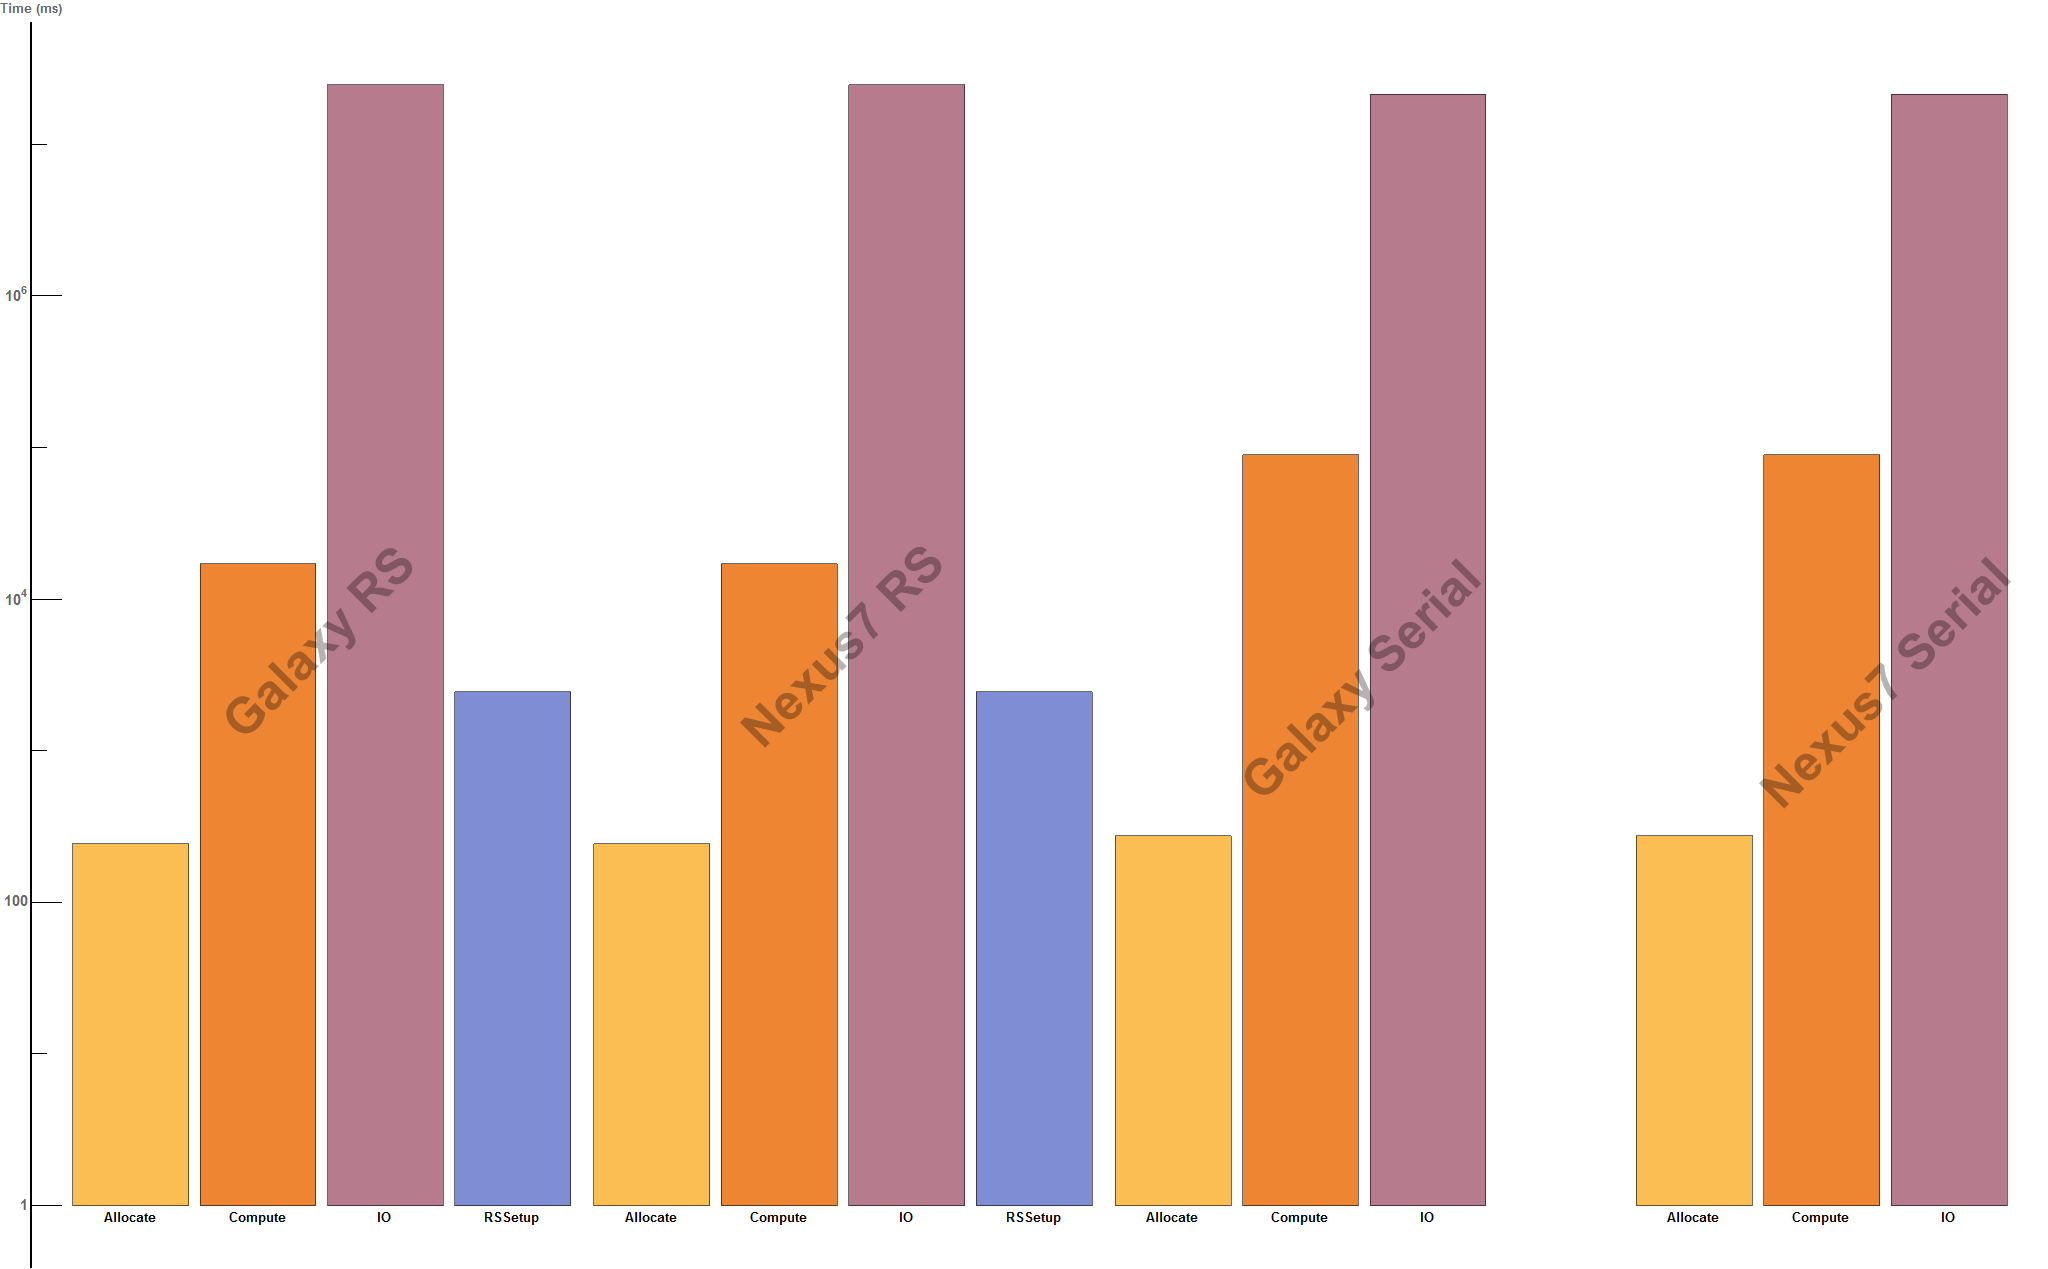
\includegraphics[scale=0.125]{Sgemm.png}
\caption{Matrix Matrix Multiplication Benchmark.}
\label{fig:sgemm}
\centering
\end{figure}



In figure~\ref{fig:stencil}, we should the results from running the stencil code across the different
  implementations.

The serial versions have an added {\tt RSSetup} time, this is either due to bad parsing of the 
  output data or an incorrect labeling of a timer in the source code.

\begin{figure}[t!]
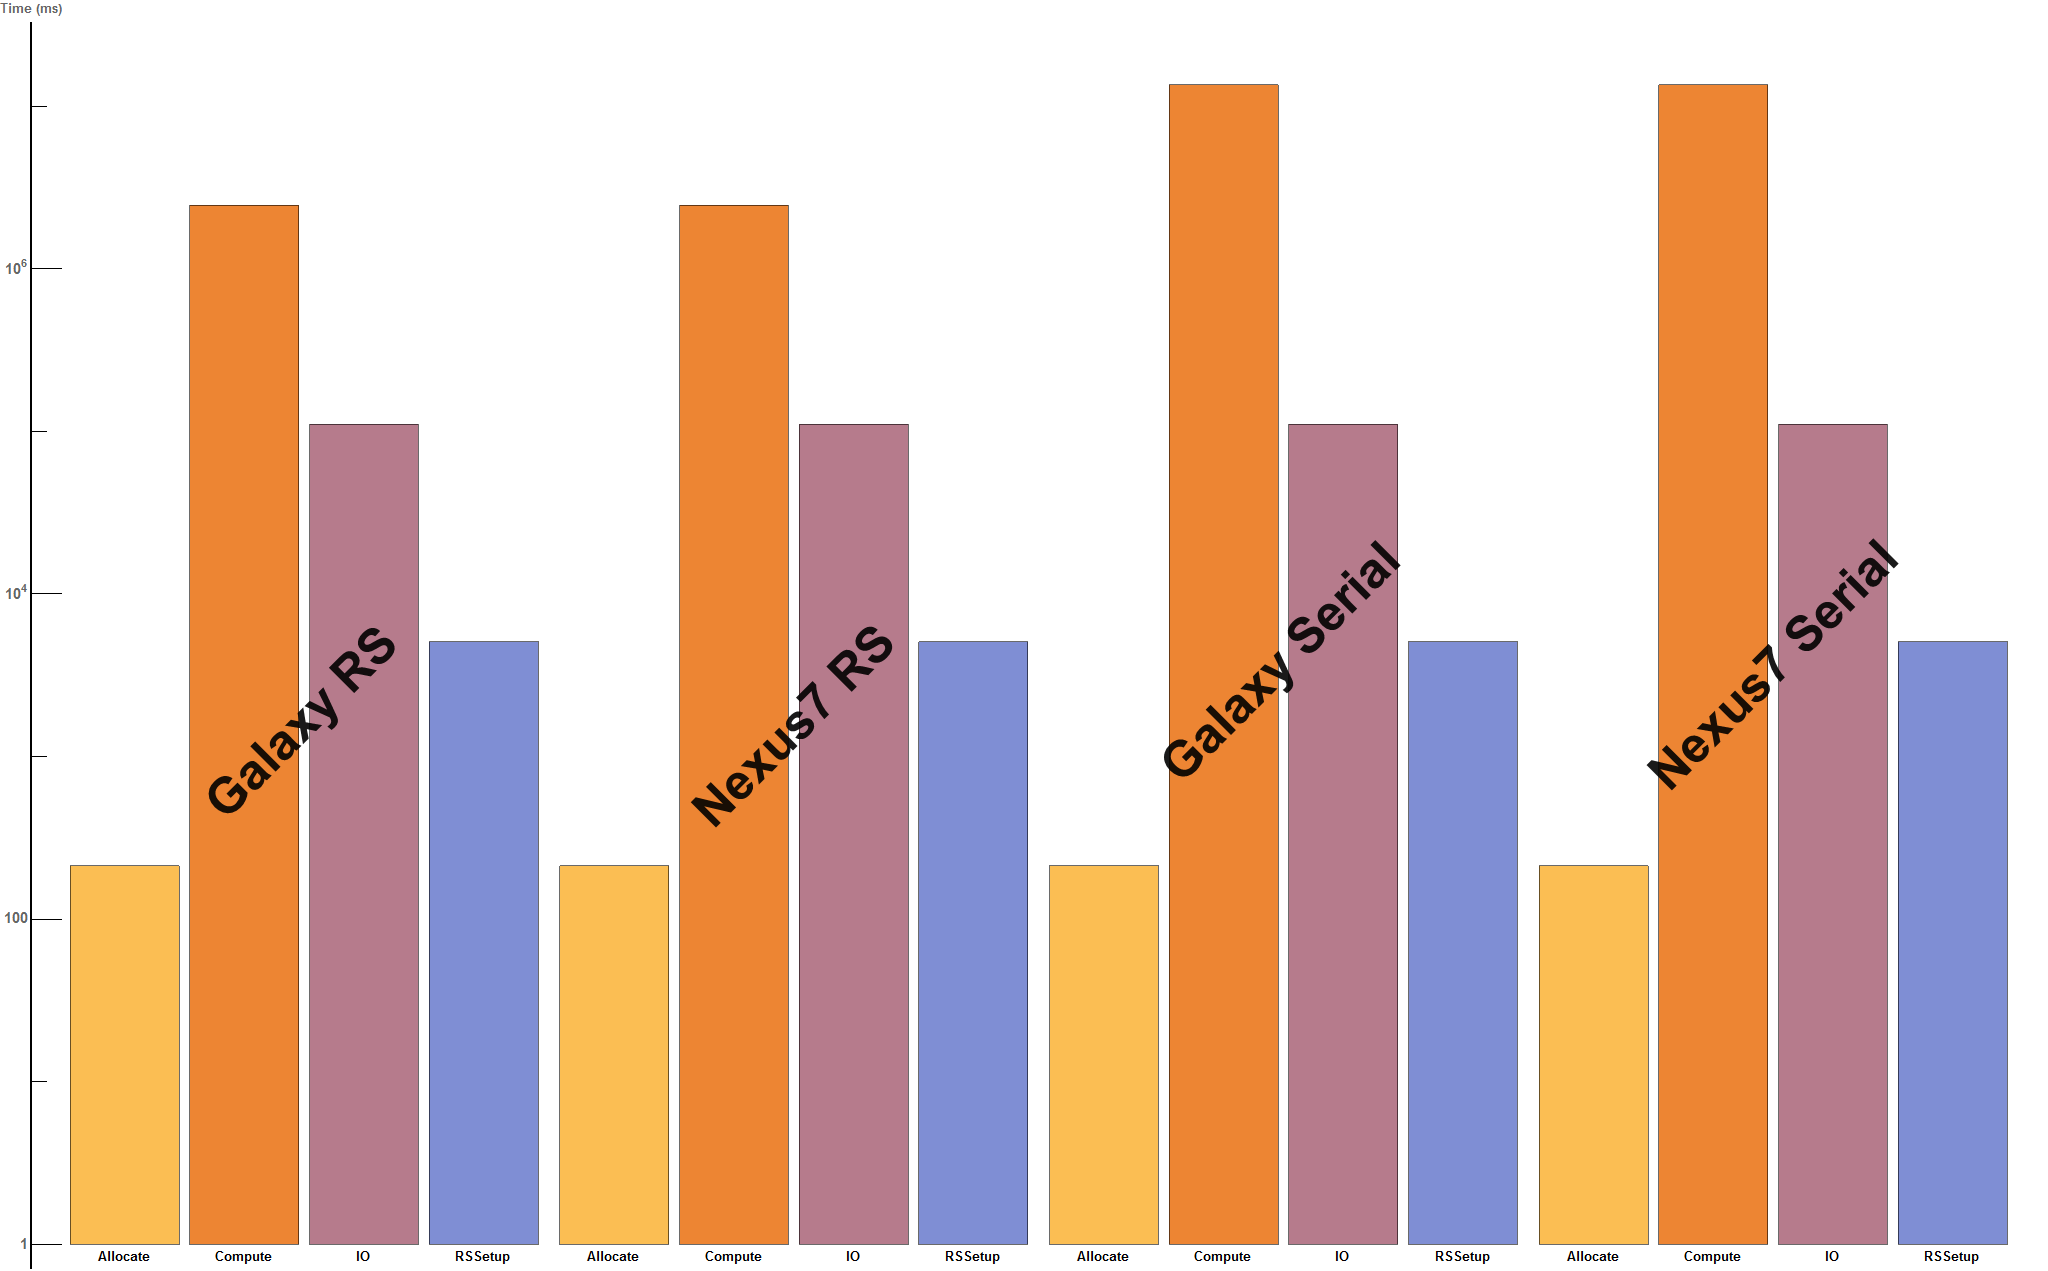
\includegraphics[scale=0.125]{Stencil.png}
\caption{Stencil Benchmark.}
\label{fig:stencil}
\centering
\end{figure}


While these graphs have the infromation, they are not presented in the clearest way.
Future work would remove the IO times from the plots, this would avoid us having to use Log scalling
  and would make some of the differences more visable.
  


\section{Related Work}
\label{sec:related}

In term of programming model, RenderScript is similar to OpenCL~\cite{OpenCL}
and CUDA. While CUDA is designed specifically for NVIDIA GPU devices, OpenCL's
goal is similar to RenderScript, which is aiming at simplifying cross-platform
parallel programming for heterogeneous systems.  In fact, Google had an option
to adopt OpenCL, since some Android hardware already has OpenCL
SDKs~\cite{OpenCL:Android}, but they opted to create RenderScript.  Google
justified the choice by arguing that they required not only performance
portability and development efficiency, but also a more intuitive programming
and distribution model.  This decision caused some frustration from the OpenCL
community \cite{androidblockopenCL} and some hardware
vendors~\cite{googlelockin} who had made big investments on OpenCL.

Since being introduced in 2008, OpenCL performance and performance portability
has been extensively evaluated.  The most common of such evaluations is OpenCL's
performance against CUDA on GPUs~\cite{fang2011comprehensive,
weber2011comparing, van2011correlating, vassilev2010comparison,
amorim2009comparing, karimi2010performance, komatsu2010evaluating}.  On
GPUs, OpenCL and CUDA have a similar platform, memory, and programming model,
thus an one-to-one analysis is possible.  Most studies~\cite{weber2011comparing,
van2011correlating, vassilev2010comparison, amorim2009comparing}, from a wide
array of domains, show that CUDA usually achieves better performance (on NVIDIA
GPUs) than OpenCL.  Another consensus among these studies is that OpenCL
provides a sufficient interface for developers to express more architectural
details to improve the performance of their applications.  For example,
studies~\cite{komatsu2010evaluating} and \cite{fang2011comprehensive} show that
most OpenCL kernels can obtain comparable performance with CUDA kernels when
properly optimized.
% In~\cite{shen2012performance}, the authors compare OpenCL
% and OpenMP in the context of application performance on multi-core CPUs using
% the Rodinia benchmark suite~\cite{che2009rodinia}.  From the study, the OpenMP
% implementations generally outperforms the OpenCL ones.  Based on this result,
% the authors picked three OpenCL worse-performed applications, compared the
% performance against OpenMP, and performed manual performance tuning.  Their
% result show that tuned OpenCL applications outperformed the OpenMP in majority
% of the test cases.

According to \cite{komatsu2010evaluating} and \cite{dolbeau2013one}, OpenCL
achieves fairly stable performance across the tested platforms. However, both
studies also illustrate some cases, in which OpenCL does not handle
architectural specifics well, such as memory layout and number of processing
cores. In order to improve the portability of applications, recent OpenCL
versions has an option to let the runtime decides the group size, i.e., the
number of concurrent threads, or wrap size in CUDA's term. However, we are not
aware of any study that evaluates the optimality of this feature.

% Compared with OpenCL, RenderScript's programming model is more restrictive, in
% the sense that it does not let developers to control the execution scheduling,
% i.e., developers do not know whether a particular region of code is going to be
% executed in a CPU or in a GPU at runtime. RenderScript also limits developers
% from expressing architectural specifics, such as the number of processing cores,
% local memory size. This study will evaluate whether hiding architectural details
% results in RenderScript incurring performance loss compared to OpenCL.

There are many recent proposals aiming at making parallel software development
easier and better utilizing multicores and GPUs available in
mobile devices. Chen et al.~\cite{6704508} introduces a new programming model,
called Android-Aparapi, which is based on the Aparapi model~\cite{Aparapi_web}
to allow Android applications to run parallel Java code on GPU via OpenCL.
Qualcomm has been developing an Android programming library and API, called
MARE (Multicore Asynchronous Runtime Environment)~\cite{MARE_qc}, to facilitate writing parallel
C code via Android Native Development Kit (NDK).
Other studies focused on further simplifying the development of RenderScript
code. In order to quickly reuse OpenCL legacy code in Android environments, Yang
et al.~\cite{yang2012o2render} presents a source-to-source translator from
OpenCL to RenderScript. The authors present several challenges of this process,
the most notable one is the differences in the execution models of the two
standards. More recently, Acosta et al.~\cite{alejandro2014performance}
proposes a parallel development framework, called Paralldroid, for improving the
parallelism of programs running in the Android platform. The framework
automatically generates parallel code in C and RenderScript based on
programmers' annotation in Java code. The results show that the auto-generated
RenderScript code often achieves higher performance than the auto-generated
Native C code.

In term of benchmarking RenderScript, study \cite{kemp2013using} compares three
different programming models, namely RenderScript, Remote CUDA (RCUDA), and C++,
of an image processing library in Android platform. The results on a Tegra 3
quad core device evidently show that RenderScript outperforms both the RCUDA and
C++ implementations. Furthermore, this performance gap increases as the size of
the input increases.  However, we are not aware of any work that provides a
systematic evaluation of RenderScript's performance and performance portability.
The only available tool that we might be able to leverage is CompuBench mobile
for RenderScript~\cite{compuBenchMobile}.  But since this benchmark is a
commercial product and does not offer source, we would not be able to perform
thorough analysis using this it.  So in this regard, we will be providing the
first open source benchmark for RenderScript that can be evaluated against
different language paradigms and hadware targets.

\section{Conclusion and Future Work}

RenderScript is awesome?

\section{Future Work}



\todo[inline]{Discuss Future Work.}


% We recommend abbrvnat bibliography style.

\bibliographystyle{abbrvnat}
\bibliography{paper}


\listoftodos
\end{document}
